\documentclass[11pt]{article}
\usepackage{amsmath,amssymb,amsthm}

\DeclareMathOperator*{\E}{\mathbb{E}}
\let\Pr\relax
\DeclareMathOperator*{\Pr}{\mathbb{P}}

\newcommand{\eps}{\varepsilon}
\newcommand{\inprod}[1]{\left\langle #1 \right\rangle}
\newcommand{\R}{\mathbb{R}}

\newcommand{\handout}[5]{
  \noindent
  \begin{center}
  \framebox{
    \vbox{
      \hbox to 5.78in { {\bf CS 224: Advanced Algorithms } \hfill #2 }
      \vspace{4mm}
      \hbox to 5.78in { {\Large \hfill #5  \hfill} }
      \vspace{2mm}
      \hbox to 5.78in { {\em #3 \hfill #4} }
    }
  }
  \end{center}
  \vspace*{4mm}
}

\newcommand{\lecture}[4]{\handout{#1}{#2}{#3}{Scribe: #4}{Lecture #1}}

\newtheorem{theorem}{Theorem}
\newtheorem{corollary}[theorem]{Corollary}
\newtheorem{lemma}[theorem]{Lemma}
\newtheorem{observation}[theorem]{Observation}
\newtheorem{proposition}[theorem]{Proposition}
\newtheorem{definition}[theorem]{Definition}
\newtheorem{claim}[theorem]{Claim}
\newtheorem{fact}[theorem]{Fact}
\newtheorem{assumption}[theorem]{Assumption}

% 1-inch margins, from fullpage.sty by H.Partl, Version 2, Dec. 15, 1988.
\topmargin 0pt
\advance \topmargin by -\headheight
\advance \topmargin by -\headsep
\textheight 8.9in
\oddsidemargin 0pt
\evensidemargin \oddsidemargin
\marginparwidth 0.5in
\textwidth 6.5in

\parindent 0in
\parskip 1.5ex

%% Custom for this file
% Diagrams
\usepackage{tikz}
\usetikzlibrary{arrows,shapes}
\tikzstyle{vertex}=[ellipse,fill=black!25,minimum size=20pt,inner sep=0pt]
\tikzstyle{edge} = [draw,thick,-]
\tikzstyle{arr} = [draw,thick,->]
\tikzstyle{darr} = [draw,thick,dashed,->]
\tikzstyle{weight} = [font=\small]
\begin{document}

\lecture{5 --- February 7, 2017}{Spring 2017}{Prof.\ Jelani Nelson}{Rohit Agrawal}


\section{Wrapping up approximate membership}
Recall that the approximate membership problem for a set $S\subset [u]$ of size
$n$ entails answering queries of the form ``is $x\in S$'', subject to the
constraint that if $x\in S$ the algorithm always returns yes, and if $x\not\in
S$ the algorithm returns yes with probability at most $\epsilon$.

Last week we saw the Bloom filter \cite{Bloom1970} which used space
$O\big(n\lg(1/\epsilon)\big)$ bits and update/query time $O\big(\lg
(1/\epsilon)\big)$. This leads to the natural question, \textbf{are these bounds
optimal?}

This was partially answered in the affirmative by Carter, Floyd, Gill,
Markowsky, and Wegman \cite{Carter1978}, who showed that static approximate
membership requires $\Omega\big(n\lg (1/\epsilon)\big)$ bits of space. They also
gave a different data structure that used space $n\lg(1/\epsilon) + O(n)$ bits.
This result was improved and partially dynamized by Arbitman, Naor, and Segev
\cite{Arbitman2010} who gave another implementation matching the space of
\cite{Carter1978}, but also supporting insertion and $O(1)$ update/query. This
result was extended to deletions by Pagh, Segev, and Wieder \cite{Pagh2013} at
the cost of achieving amortized and expected time bounds rather than worst-case.

\section{Dynamic Dictionary and Cuckoo Hashing}
The dynamic dictionary problem (without deletions) asks us to maintain the set
$\mathcal{S} = S\times V$ with $S\subseteq [u]$ a set of keys, subject to the
following operations:
\begin{itemize}
\item $\mathtt{insert}(x, v)$: add $(x, v)$ to $\mathcal{S}$, removing any
 other mapping of $x$.
\item $\mathtt{query}(x)$: returns the most recent $v$ stored with a call
to $\mathtt{insert}(x, v)$.
\end{itemize}


\textbf{Cuckoo hashing}, introduced by Pagh and Rodler \cite{Pagh2004}, solves
this problem. The structure stores two random hash functions $h, g: [u] \to [m]$
where $m = c\cdot n$ (with $c = 4$ sufficient), and an array $A[1\dotsc m]$ that
stores items. The structure will maintain the invariant that the entry $x$ will
always be stored in either $A[h(x)]$ or $A[g(x)]$, so that queries will take
constant time.

Hence, the main procedure of interest is insertion. Upon a call to
$\mathtt{insert}(x, v)$, we consider four cases:
\begin{itemize}
\item $A[h(x)]$ is empty. This case is trivial, and we simply put $(x, v)$
 in $A[h(x)]$.
\item In the other three cases, $A[h(x)]$ is already full. In all cases, we will
set $A[h(x)] = (x, v)$ and place the old element in $A[h(x)]$ (suppose it is
$(y, z)$) in the position given by the other hash function of $y$. For example,
if $h(x) = h(y)$, we will move $(y, z)$ to $A[g(y)]$, and if $h(x) = g(y)$ we
will move $(y, z)$ to $A[h(y)]$. As the new location for $y$ might also be
occupied, we iterate this process.

There are three different ways this iteration can go.
\begin{itemize}
\item There are no cycles, and the shifts form a path.
\[
  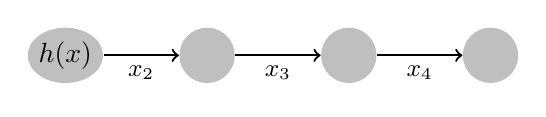
\begin{tikzpicture}[scale=1.8, auto,swap]
    \foreach \pos/\name/\val in {{(0,0)/a/h(x)}, {(1,0)/b/},
    {(2,0)/c/},{(3,0)/d/}}
        \node[vertex] (\name) at \pos {$\val$};

    \foreach \source/ \dest /\weight in
    {a/b/x_2,b/c/x_3,c/d/x_4}
        \path[arr] (\source) -- node[weight] {$\weight$} (\dest);
\end{tikzpicture}
\]

In this case, we shift around some items but eventually find an empty slot.

\item There is a cycle formed by shifting around the positions starting with
$h(x)$, so we try again with $g(x)$ and succeed since it forms a path.

\[
  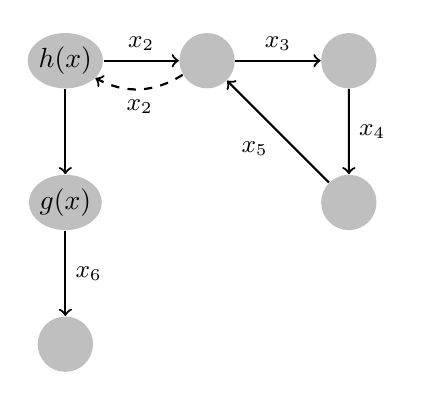
\begin{tikzpicture}[scale=1.8, auto]
    \foreach \pos/\name/\val in {{(0,0)/a/h(x)}, {(1,0)/b/},
    {(2,0)/c/},{(2,-1)/d/},{(0,-1)/e/g(x)},{(0,-2)/f/}}
        \node[vertex] (\name) at \pos {$\val$};

    \foreach \source/ \dest /\weight /\shouldswap in {a/b/x_2/,b/c/x_3/,
    c/d/x_4/,d/b/x_5/,a/e//,e/f/x_6/}
        \path[arr,\shouldswap] (\source) -- node[weight] {$\weight$} (\dest);

    \path[darr] (b) to [bend left] node[weight] {$x_2$} (a);
\end{tikzpicture}
\]

In this case, we shift around some items but eventually find an empty slot.

\item There is a cycle formed by shifting around the positions  starting with
$h(x)$, so we try again with $g(x)$ and find another cycle.

\[
  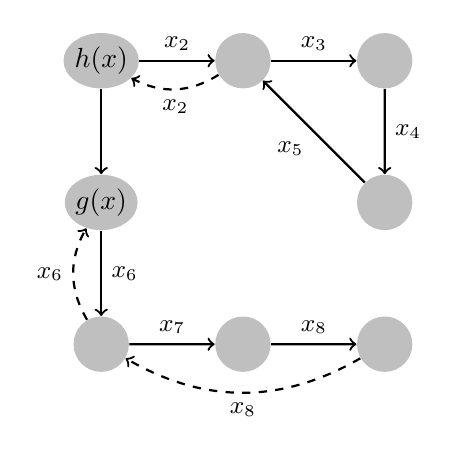
\begin{tikzpicture}[scale=1.8, auto]
    \foreach \pos/\name/\val in {{(0,0)/a/h(x)}, {(1,0)/b/},
    {(2,0)/c/},{(2,-1)/d/},{(0,-1)/e/g(x)},{(0,-2)/f/},
    {(1,-2)/g/},{(2,-2)/h/}}
        \node[vertex] (\name) at \pos {$\val$};

    \foreach \source/ \dest /\weight /\shouldswap in {a/b/x_2/,b/c/x_3/,
    c/d/x_4/,d/b/x_5/,a/e//,e/f/x_6/,f/g/x_7/,g/h/x_8/}
        \path[arr,\shouldswap] (\source) -- node[weight] {$\weight$} (\dest);

    \path[darr] (b) to [bend left] node[weight] {$x_2$} (a);
    \path[darr] (h) to [bend left] node[weight] {$x_8$} (f);
    \path[darr] (f) to [bend left] node[weight] {$x_6$} (e);
\end{tikzpicture}
\]

In this case, we shift around some items indefinitely, and \emph{never} find
an empty slot! To address this, if we encounter a double cycle like in this
case, we abandon the current Cuckoo hash, choose two new random hash functions,
and re-insert all the items into that data structure. We will show that this
happens so rarely we can afford to do such an expensive operation.
\end{itemize}
\end{itemize}
There is one additional subtlety involved in insertion: we keep a counter of
number of shuffles, and if we ever reach $50\lg n$, we give up on the current
structure and try again as in the last case of a double cycle.

\subsection{Runtime analysis}

It remains to do an analysis of the expected time to do an insertion. Let $T$ be
the random variable representing the time to do an insertion. Let $P_k$ be an
indicator for the random variable that the shuffling from the insertion forms a
path (case $2$ above), and furthermore that the path is of length at least $k$.
Similarly, let $C_k$ be the indicator for the random variable that the shuffling
from the insertion forms a single cycle (case $3$ above), and furthermore that
the total number of distinct edges traversed is at least $k$. Similarly, let
$D_k$ be the indicator for the random variable that the shuffling from the
insertion forms a double cycle (case $4$ above), and furthermore that the total
number of distinct edges traversed is at least $k$.

With this terminology, we can bound
\[
\E[T] \leq \E\left[\sum_{k=1}^{\infty} P_k + \sum_{k=1}^{\infty} C_k\right] +
n\cdot \E[T] \cdot \left[\sum_{k=1}^{\infty} \Pr(D_k = 1)
+ \Pr(\text{more than $50\lg n$ shuffles})\right]
\]
where the last term includes giving up and rebuilding. If $\alpha$ is the
probability of rebuilding, then rearranging gives
\[\E[T] \leq \frac{1}{1 - \alpha\cdot n} \left[\sum_{k=1}^\infty
\E[P_k] + \sum_{k=1}^{\infty} \E[C_k]\right].
\]
We will show that the denominator is $1 - o(1)$ and the term in brackets is
$O(1)$ so that $\E[T] = O(1)$.

Let's bound $\Pr(P_k = 1)$ for each $k$. Fix a particular path (i.e. hash
locations/vertices $y_1, y_2, \dotsc, y_{k+1})$ and edges $x_2, x_3, \dotsc,
x_{k+1}$. The probability that $h(x) = y_1$ is $m^{-1}$, and for each edge $x_i$
the probability that $\{g(x_i), h(x_i)\} = \{y_{i-1}, y_i\}$ is at most
$2m^{-2}$ (one copy of $m^{-2}$ for each ordering of $(g, h)$ and $(h, g)$).
Hence, the probability of the particular path is at most $m^{-1}\cdot
(2m^{-2})^k$. There are at most $m^{k+1}$ possible choices of vertices and $n^k$
choices of edges, so a union bound implies the probability of seeing any cycle
of length $k$ is
\[\E[P_k] = \Pr(P_k = 1) \leq \frac{1}{m}\left(\frac{2}{m^2}\right)^k\cdot
m^{k+1}\cdot n^k = \left(\frac{2}{c}\right)^k\]
as $m = c\cdot n$. In particular, if $c = 4$, we have that
\[\E\left[\sum_{k=1}^{\infty} P_k \right] \leq \sum_{k=1}^{\infty}
\left(\frac{2}{4}\right)^k = 1.\]

What about $\Pr(C_k = 1)$? This is mostly analogous, and is left as an exercise.
Hint: it is possible to categorize the edges depending on whether the edge
occurs before or after reaching the cycle. At least one of these subpaths has
length at least $k/2$, and a similar analysis as above holds.

What about $\Pr(D_k = 1)$? A double cycle with $k$ distinct edges has
$k - 1$ distinct vertices. Fix these $k - 1$ vertices and $k$ edges. The
probability that $h(x)$ and $g(x)$ are correct is at most $m^{-2}$, and for
each of the other $k - 1$ edges the probability is at most $2m^{-2}$. Hence,
since there are at most $m^{k-1}$ possible vertex choices and $n^{k-1}$ possible
other edge choices, by a union bound the probability of any double cycle of
length $k$ is at most
\[\Pr(D_k = 1) \leq \frac{1}{m^2}\cdot \left(\frac{2}{m^2}\right)^{k-1}\cdot
m^{k-1}\cdot n^{k-1} = \left(\frac{2}{c}\right)^k \cdot \frac{1}{n^2}\]
so that
\[\sum_{k=1}^{\infty} \Pr(D_k = 1) = \Theta\left(\frac{1}{n^2}\right).\]

Finally, what is the probability of reaching $50\lg n$ shuffles? This is
analogous to the analysis of $P_k$ and $C_k$ analysis with the single large term
$k^* = 50\lg n$. It is an exercise to fill out the details, but again the
probability will be $(2c^{-1})^{\Theta(\lg n)} = o(1)$.

Hence, we have that
\[\E[T] \leq \frac{1}{1 - \alpha\cdot n} \left[\sum_{k=1}^\infty
\E[P_k] + \sum_{k=1}^{\infty} \E[C_k]\right]
\leq \frac{1}{1 - o(1)}[O(1) + O(1)]  = O(1)
\]
as desired.

Note that this analysis assumed that $h$ and $g$ were random hash functions. It
is an exercise to show that if $h$ and $g$ are drawn from a $\Theta(\lg n)$-wise
independent family, then expected time per insertion is still $\Theta(1)$. It is
not known if this much independence is necessary, but partial progress was made
by Cohen and Kane \cite{Cohen2009} who constructed a $5$-wise independent
family which does not give expected constant time.

\section{Approximate static dictionary}
Consider the problem of \emph{approximate static dictionary}, which requires
maintaining $S\times \{0,1\}^r$ for $S \subseteq [u]$ a set of keys and
$\{0,1\}^r$ the set of values, subject to:
\begin{itemize}
\item $\mathtt{query}(x)$: Returns the associated $r$-bit string if $x\in
S$, and returns an arbitrary string if $x\not\in S$.
\end{itemize}

This differs from non-approximate static dictionary as the behavior when
$x\not\in S$ can be arbitrary rather than reporting that $x\not\in S$. Known
solutions to non-approximate static dictionary (for example, using $2$-level
perfect hashing as covered in CS125) have parameters $O\big(n\cdot (r + \lg
u)\big)$ bits of memory and $O(1)$ query time.

The use of approximation allows better space bounds, as in the \textbf{Bloomier
filters} of Chazelle, Kilian, Rubinfeld, and Tal \cite{Chazelle2004} which solve
approximate static dictionary with an $r$-bit string using $O(nr)$ bits and
$O(1)$ query time. The name invokes the Bloom filter, which can be thought of as
an approximate static dictionary with $r = 1$ with the value being an indicator
of whether the element is in the set.

We will present a different data structure based on Cuckoo hashing that matches
the same bounds.

First, define the \emph{Cuckoo graph} associated to a Cuckoo hash as the graph
$G$ with $m$ vertices, labelled by locations in the array $A$, and $n$
(undirected) edges labelled by the elements in $S$, with an edge $\big(h(x),
g(x)\big)$ for each $x\in S$.

Our data structure now works as follows, for preprocessing, store the set $S$ in
a Cuckoo hash. If the associated Cuckoo graph $G$ is not a forest, abandon the
Cuckoo hash and try again (remember that the Cuckoo hash is randomized). Repeat
until the Cuckoo graph is acyclic (we will show this takes $O(1)$ attempts in
expectation). Now, we have a Cuckoo graph $G$ which is a forest. For each tree
in $G$, consider an arbitrary node as the root, and associate to it the $r$-bit
zero vector. Recall that edges in the Cuckoo graph are labelled by indices of
$A$, and edges by elements in $S$. For each vertex $v$ in the tree with edge $x$
to its parent, associate $A[parent(v)]\oplus key(x)$ to $v$. This is illustrated
in Figure \ref{fig:cuckoograph}.

\begin{figure}[htbp]
\centering
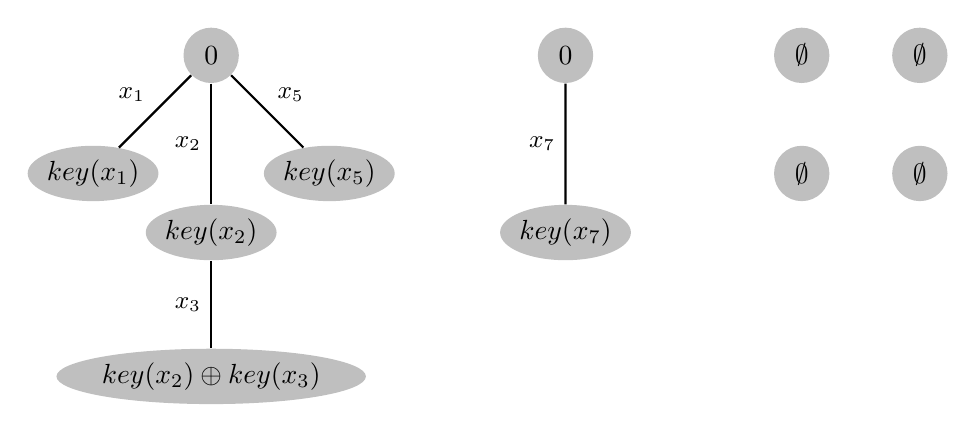
\begin{tikzpicture}[scale=1.5, auto,swap]
    \foreach \pos/\name/\val in {{(0,0)/a/0}, {(-1,-1)/b/key(x_1)},
    {(1,-1)/c/key(x_5)},{(0,-1.5)/d/key(x_2)}, {(0,-e)/e/key(x_2)\oplus
    key(x_3)}, {(3,0)/f/0}, {(3,-1.5)/g/key(x_7)}, {(5,0)/h/\emptyset},
    {(6,0)/i/\emptyset}, {(5,-1)/j/\emptyset}, {(6,-1)/k/\emptyset}}
        \node[vertex] (\name) at \pos {$\val$};
    \foreach \source/ \dest /\weight in {a/b/x_1,c/a/x_5,a/d/x_2,d/e/x_3,
    f/g/x_7}
        \path[edge] (\source) -- node[weight] {$\weight$} (\dest);
\end{tikzpicture}
\caption{Cuckoo graph and labelling}
\label{fig:cuckoograph}
\end{figure}

Queries in the graph are then answered by taking the xor of the associated
values of the nodes $h(x)$ and $g(x)$ in $G$, and hence can be done in constant
time.  We don't need to store isolated vertices or the keys themselves, so
(ignoring the hash functions $h$ and $g$), the total space used is $r$ bits
per each of at most $2n$ nodes, for total space $O(n\cdot r)$ bits as desired.
Note that this analysis ignored the $O(n\lg u)$ bits needed to store the fully
independent hash functions, it will be an exercise to show that this can be done
in a space efficient manner using a $\Theta(\lg n)$-independent family.

All that remains is to show that in expectation, we only need $O(1)$ iterations
to find a Cuckoo hash with acyclic Cuckoo graph. To do this, we need to bound
the probability that the Cuckoo graph contains a cycle. There are two types of
cycles: cycles of length $1$ in which $h(x) = g(x)$ for some $x$, and cycles of
length at least $2$. For fixed $x$ and value $y$, the probability that $h(x) =
g(x) = y$ is $m^{-2}$, so by a union bound over the $n$ values of $x$ and $m$
values of $y$, the probability of a single element cycle is at most $n\cdot m
\cdot m^{-2} = c^{-1}$ as $m = c\cdot n$. For longer cycles of length $t\geq 2$,
by fixing the vertices $y_1,y_2,\dotsc, y_t$ and edges $x_1, x_2, \dotsc, x_t$,
the probability of each edge being in the appropriate place is at most $2m^{-2}$
(one copy of $m^{-2}$ for each order of $(g, h)$ and $(h, g)$). Hence, by a
union bound over the at most $m^t$ ordered vertices and $n^t$ edge labels, the
probability of a cycle of length $t$ is at most $(2m^{-2})^t\cdot m^t\cdot n^t =
(2c^{-1})^t$. Hence, the probability there is a cycle is at most
\[
  \Pr(\exists\text{ a cycle}) \leq \frac{1}{c} +
  \sum_{t=2}^{\infty} \left(\frac{2}{c}\right)^t
   = \frac{1}{c} + \frac{(2/c)^2}{1 - 2/c}
\]
which if $c = 4$ is equal to $3/4$. Hence, the probability there is no cycle is
at least $1/4$, and thus the expected number of tries to get an acyclic Cuckoo
graph is at most $(1/4)^{-1} = 4 = O(1)$ as desired.

Note that this proof used full independence, as mentioned before it will be an
exercise to reduce this to using $\Theta(\lg n)$-wise independence.

\bibliographystyle{alpha}

\newcommand{\etalchar}[1]{$^{#1}$}
\begin{thebibliography}{CKRT04}

\bibitem[ANS10]{Arbitman2010}
Yuriy Arbitman, Moni Naor, and Gil Segev.
\newblock Backyard cuckoo hashing: Constant worst-case operations with a
  succinct representation.
\newblock In {\em 2010 IEEE 51st Annual Symposium on Foundations of Computer
  Science}, pages 787--796, Oct 2010.

\bibitem[Blo70]{Bloom1970}
Burton~H. Bloom.
\newblock Space/time trade-offs in hash coding with allowable errors.
\newblock {\em Commun. ACM}, 13(7):422--426, July 1970.

\bibitem[CFG{\etalchar{+}}78]{Carter1978}
Larry Carter, Robert Floyd, John Gill, George Markowsky, and Mark Wegman.
\newblock Exact and approximate membership testers.
\newblock In {\em Proceedings of the Tenth Annual ACM Symposium on Theory of
  Computing}, STOC '78, pages 59--65, New York, NY, USA, 1978. ACM.

\bibitem[CK09]{Cohen2009}
Jeffrey Cohen and Daniel~M. Kane.
\newblock Bounds on the independence required for cuckoo hashing.
\newblock Manuscript submitted to ACM Transactions on Algorithms, 2009.

\bibitem[CKRT04]{Chazelle2004}
Bernard Chazelle, Joe Kilian, Ronitt Rubinfeld, and Ayellet Tal.
\newblock The {B}loomier filter: An efficient data structure for static support
  lookup tables.
\newblock In {\em Proceedings of the Fifteenth Annual ACM-SIAM Symposium on
  Discrete Algorithms}, SODA '04, pages 30--39, Philadelphia, PA, USA, 2004.
  Society for Industrial and Applied Mathematics.

\bibitem[PR04]{Pagh2004}
Rasmus Pagh and Flemming~Friche Rodler.
\newblock Cuckoo hashing.
\newblock {\em J. Algorithms}, 51(2):122--144, May 2004.

\bibitem[PSW13]{Pagh2013}
Rasmus Pagh, Gil Segev, and Udi Wieder.
\newblock How to approximate a set without knowing its size in advance.
\newblock In {\em 2013 IEEE 54th Annual Symposium on Foundations of Computer
  Science}, pages 80--89, Oct 2013.

\end{thebibliography}


\end{document}
